\documentclass[12pt]{article}
\usepackage{tikz}
\usetikzlibrary{bayesnet}
\usepackage{amsmath}
\DeclareMathOperator*{\argmax}{arg\,max}
\DeclareMathOperator*{\erf}{erf}
\begin{document}

\section*{Divisive Normalization Notes}

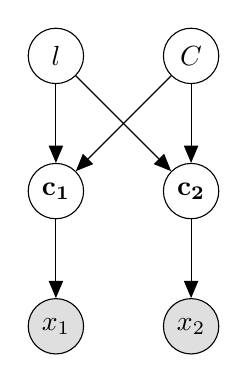
\begin{tikzpicture}

  % Define nodes
  \node[obs]                               (x_1) {$x_1$};
  \node[obs, right=of x_1]         (x_2) {$x_2$};
  \node[latent, above=of x_1] (c_1) {$\mathbf{c_1}$};
  \node[latent, above=of x_2]  (c_2) {$\mathbf{c_2}$};
  \node[latent, above=of c_2]   (C) {$C$};
  \node[latent, above=of c_1]   (l) {$l$};

  % Connect the nodes
  \edge {C,l} {c_2} ; 
  \edge {C,l} {c_1} ; 
  \edge {c_1} {x_1} ; 
  \edge {c_2} {x_2} ; 

\end{tikzpicture} 
\\
\\
C is categorical variable for condition\\
$l$ is level of background light\\
$c_i$ is log contrast of grating i\\
$x_i$ is noisy log measurement of $c_i$\\
$p(C=1) = 0.25$\\
$p(C=2) = 0.25 (c_1 > 0)$\\
$p(C=3) = 0.25 (c_2 > 0)$\\
$p(C=4) = 0.25 (c_1 and c_2 > 0)$\\
$l = k$\\
$p(c_1|C=1$ or $3, l) = \delta(c_1)$\\
$p(c_1|C= 2$ or $4, l) = \mathcal{N}(c_1; l, \sigma_c^2)$\\
$p(c_2|C=1$ or $2, l) = \delta(c_2)$\\
$p(c_2|C=3$ or $4, l) = \mathcal{N}(c_2; l, \sigma_c^2)$\\
$p(x_i|c_i) = \mathcal{N}(x_i; c_i, \sigma^2)$
\begin{equation}
\begin{aligned}
p(c_1, c_2|x_1, x_2) &\propto p(x_1, x_2, c_1, c_2) \\ 
& =  \sum\limits_{C} \int p(x_1, x_2, c_1, c_2, l, C) dl\\
& = \sum\limits_{C} \int p(x_1|c_1)p(x_2|c_2) p(c_1, c_2, l, C) dl \\
& = \int p(x_1|c_1)p(x_2|c_2) p(c_1, c_2, l, C=1) dl \\
&\phantom{{}=1}+ \int p(x_1|c_1)p(x_2|c_2) p(c_1, c_2, l, C=2) dl\\
&\phantom{{}=1}+ \int p(x_1|c_1)p(x_2|c_2) p(c_1, c_2, l, C=3 dl\\
&\phantom{{}=1}+ \int p(x_1|c_1)p(x_2|c_2) p(c_1, c_2, l, C=4) dl\\
& = p(x_1|c_1)p(x_2|c_2) \delta(c_2)\delta(c_1) \\
&\phantom{{}=1} + \int p(x_1|c_1)p(x_2|c_2) \delta(c_2) \mathcal{N}(c_1; l, \sigma_c^2)dl \\
&\phantom{{}=1} + \int p(x_1|c_1)p(x_2|c_2) \delta(c_1) \mathcal{N}(c_2; l, \sigma_c^2)dl \\
&\phantom{{}=1} + \int p(x_1|c_1)p(x_2|c_2) \mathcal{N}(c_1; l, \sigma_c^2) \mathcal{N}(c_2; l, \sigma_c^2)dl \\
& = p(x_1|c_1)p(x_2|c_2) \delta(c_2)\delta(c_1) + p(x_1|c_1)p(x_2|c_2) \delta(c_1)\\
& \phantom{{}=1} + p(x_1|c_1)p(x_2|c_2) \delta(c_2) +  \int p(x_1|c_1)p(x_2|c_2)\mathcal{N}(l; \frac{c_1 + c_2}{2}, 2\sigma_c^2)\mathcal{N}(c_1; c_2, 2\sigma_c^2) \\
& = \mathcal{N}(x_1; c_1, \sigma^2)\mathcal{N}(x_2; c_2, \sigma^2)\delta(c_1)\delta(c_2) + \mathcal{N}(x_1; c_1, \sigma^2)\mathcal{N}(x_2; c_2, \sigma^2)\delta(c_1) \\
& \phantom{{}=1} + \mathcal{N}(x_1; c_1, \sigma^2)\mathcal{N}(x_2; c_2, \sigma^2)\delta(c_2)  + \mathcal{N}(x_1; c_1, \sigma^2)\mathcal{N}(x_2; c_2, \sigma^2)\mathcal{N}(c_1; c_2, 2\sigma_c^2) \\
\end{aligned}
\end{equation}

Normalization term(A):
\begin{equation}
\begin{aligned}
A & = \iint [p(x_1|c_1)p(x_2|c_2) \delta(c_2)\delta(c_1) + p(x_1|c_1)p(x_2|c_2) \delta(c_1) \\
& \phantom{{}=1} + p(x_1|c_1)p(x_2|c_2) \delta(c_2) +  p(x_1|c_1)p(x_2|c_2)\mathcal{N}(c_1; c_2, 2\sigma_c^2)]dc_1dc_2 \\
& = p(x_1|c_1=0)p(x_2|c_2=0) + p(x_1|c_1=0) + p(x_2|c_2=0) \\
& \phantom{{}=1} + \int[\mathcal{N}(x_1; c_1, \sigma_c^2) \mathcal{N}(x_2; c_1, \sigma^2 + 2\sigma_c^2)]dc_1\\
& = \mathcal{N}(x_1; 0, \sigma^2)\mathcal{N}(x_2; 0, \sigma^2) + \mathcal{N}(x_1; 0, \sigma^2) +\mathcal{N}(x_2; 0, \sigma^2) + \mathcal{N}(x_1; x_2, 2\sigma^2 + 2\sigma_c^2)
\end{aligned}
\end{equation}

\begin{equation}
\begin{aligned}
\left[\begin{array}{c}
\hat{c_1}\\ \hat{c_2}
\end{array}\right]
= \iint \left[\begin{array}{c}
c_1\\ c_2
\end{array}\right]
p(c_1, c_2|x_1, x_2) dc_1dc_2
\end{aligned}
\end{equation}

\begin{equation}
\begin{aligned}
\hat{c_1} & = \frac{1}{A} \iint c_1 p(x_1|c_1) p(x_2|c_2)[\delta(c_1)\delta(c_2) + \delta(c_1) +  \delta(c_2) + \mathcal{N}(c_1; c_2, 2\sigma_c^2)] dc_1dc_2 \\
& \propto \int c_1 p(x_1|c_1) [p(x_2|c_2=0)\delta(c_1) + \delta(c_1) + p(x_2|c_2=0) + \mathcal{N}(x_2; c_1, \sigma^2 + 2\sigma_c^2)]dc_1 \\
& = x_1\mathcal{N}(x_2; 0, \sigma^2) + \mathcal{N}(x_1; x_2, 2\sigma^2 + 2\sigma_c^2) \frac{\frac{x_1}{\sigma^2} + \frac{x_2}{\sigma^2 + 2\sigma_c^2}}{\frac{1}{\sigma^2} + \frac{1}{\sigma^2 + 2\sigma_c^2}} \\
& \frac{x_1\mathcal{N}(x_2; 0, \sigma^2) + \mathcal{N}(x_1; x_2, 2\sigma^2 + 2\sigma_c^2) \frac{\frac{x_1}{\sigma^2} + \frac{x_2}{\sigma^2 + 2\sigma_c^2}}{\frac{1}{\sigma^2} + \frac{1}{\sigma^2 + 2\sigma_c^2}}}{\mathcal{N}(x_1; 0, \sigma^2)\mathcal{N}(x_2; 0, \sigma^2) + \mathcal{N}(x_1; 0, \sigma^2) +\mathcal{N}(x_2; 0, \sigma^2) + \mathcal{N}(x_1; x_2, 2\sigma^2 + 2\sigma_c^2)}
\end{aligned}
\end{equation}

\begin{equation}
\begin{aligned}
\hat{c_2} & = \frac{1}{A} \iint c_2 p(x_1|c_1) p(x_2|c_2)[\delta(c_1)\delta(c_2) + \delta(c_1) +  \delta(c_2) + \mathcal{N}(c_1; c_2, 2\sigma_c^2)] dc_1dc_2 \\
& \propto \int c_2 p(x_2|c_2) [p(x_1|c_1=0)\delta(c_2) + \delta(c_2) + p(x_1|N=c_2) + \mathcal{N}(x_1; c_2, \sigma^2 + 2\sigma_c^2)]dc_2 \\
& = x_2\mathcal{N}(x_1; 0, \sigma_c^2) + \mathcal{N}(x_2; x_1, 2\sigma^2 + 2\sigma_c^2) \frac{\frac{x_2}{\sigma^2} + \frac{x_1}{\sigma^2 + 2\sigma_c^2}}{\frac{1}{\sigma^2} + \frac{1}{\sigma^2 + 2\sigma_c^2}}\\
& \frac{x_2\mathcal{N}(x_1; 0, \sigma_c^2) + \mathcal{N}(x_2; x_1, 2\sigma^2 + 2\sigma_c^2) \frac{\frac{x_2}{\sigma^2} + \frac{x_1}{\sigma^2 + 2\sigma_c^2}}{\frac{1}{\sigma^2} + \frac{1}{\sigma^2 + 2\sigma_c^2}}}{\mathcal{N}(x_1; 0, \sigma^2)\mathcal{N}(x_2; 0, \sigma^2) + \mathcal{N}(x_1; 0, \sigma^2) +\mathcal{N}(x_2; 0, \sigma^2) + \mathcal{N}(x_1; x_2, 2\sigma^2 + 2\sigma_c^2)}
\end{aligned}
\end{equation}

\begin{tabular}{ l | c | r }
	& Our Model & Heeger Model \\ \hline
	R & $\hat{c_1}G_1 + \hat{c_2}G_2$ & $\frac{c_1^nG_1 + c_2^nG_2}{c_{50}^n + (c_1^2 + c_2^2)^{\frac{n}{2}}}$ \\ \hline
	$w_1$ & $\frac{x_1\mathcal{N}(x_2; 0, \sigma^2) + \mathcal{N}(x_1; x_2, 2\sigma^2 + 2\sigma_c^2) \frac{\frac{x_1}{\sigma^2} + \frac{x_2}{\sigma^2 + 2\sigma_c^2}}{\frac{1}{\sigma^2} + \frac{1}{\sigma^2 + 2\sigma_c^2}}}{\mathcal{N}(x_1; 0, \sigma^2)\mathcal{N}(x_2; 0, \sigma^2) + \mathcal{N}(x_1; 0, \sigma^2) +\mathcal{N}(x_2; 0, \sigma^2) + \mathcal{N}(x_1; x_2, 2\sigma^2 + 2\sigma_c^2)}$ & $\frac{c_1^n}{c_{50}^n + (c_1^2 + c_2^2)^{\frac{n}{2}}}$ \\
\end{tabular}\\
\\
\\

\iffalse
Our Model: 

$R \approx \hat{c_1}G_1 + \hat{c_2}G_2$\\

if $x_2 \approx 0$, $x_1 >> 0$) then
\begin{equation}
\begin{aligned}
\hat{c_1} & = x_1\\
\hat{c_2} & = 0\\
R = x_1G_1
\end{aligned}
\end{equation}

if $x_1 \approx 0$, $x_1 >> 0$) then
\begin{equation}
\begin{aligned}
\hat{c_1} & = 0\\
\hat{c_2} & = x_2\\
R = x_2G_2
\end{aligned}
\end{equation}

if $x_2 \approx x_1 > 0$) then
\begin{equation}
\begin{aligned}
\hat{c_1} & = \frac{\frac{x_1}{\sigma^2} + \frac{x_2}{\sigma^2 + 2\sigma_c^2}}{\frac{1}{\sigma^2} + \frac{1}{\sigma^2 + 2\sigma_c^2}}\\
\hat{c_2} & = \frac{\frac{x_2}{\sigma^2} + \frac{x_1}{\sigma^2 + 2\sigma_c^2}}{\frac{1}{\sigma^2} + \frac{1}{\sigma^2 + 2\sigma_c^2}}\\
R = \frac{\frac{x_1}{\sigma^2} + \frac{x_2}{\sigma^2 + 2\sigma_c^2}}{\frac{1}{\sigma^2} + \frac{1}{\sigma^2 + 2\sigma_c^2}}G_1 + \frac{\frac{x_2}{\sigma^2} + \frac{x_1}{\sigma^2 + 2\sigma_c^2}}{\frac{1}{\sigma^2} + \frac{1}{\sigma^2 + 2\sigma_c^2}}G_2
\end{aligned}
\end{equation}\\

Heeger Model:\\

$R = \frac{c_1^nG_1 + c_2^nG_2}{c_{50}^n + (c_1^2 + c_2^2)^{\frac{n}{2}}}$\\

$c_{50} = $ semisaturation contrast $ = 13.1 +- 4.2$\\

$n = 1.5 +- 0.13$\\

$\sigma = 19 +- 2.1$\\

if $c_1 >> c_2$ then
\begin{equation}
\begin{aligned}
\hat{c_1} & = G_1\\
\hat{c_2} & = 0\\
\end{aligned}
\end{equation}

if $c_1 \approx c_2$ then
\begin{equation}
\begin{aligned}
\hat{c_1} & = \frac{2G}{c_{50}^n + 2G^{\frac{n}{2}}}\\
\hat{c_2} & = \frac{2G}{c_{50}^n + 2G^{\frac{n}{2}}}\\
\end{aligned}
\end{equation}
\\

\fi

Weiji's New Model:
\\
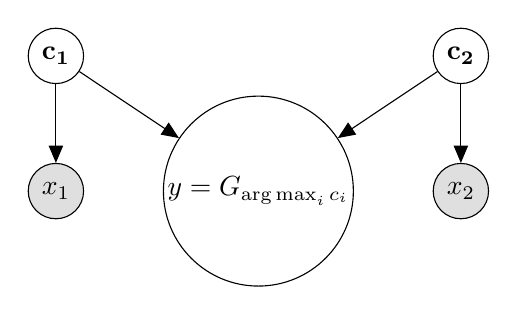
\begin{tikzpicture}

  % Define nodes
  \node[obs]                              (x_1) {$x_1$};
  \node[latent, right=of x_1]   (c_max) {$y = G_{\argmax_i c_i}$};
  \node[obs, right=of c_max]         (x_2) {$x_2$};
  \node[latent, above=of x_1] (c_1) {$\mathbf{c_1}$};
  \node[latent, above=of x_2]  (c_2) {$\mathbf{c_2}$};

  % Connect the nodes
  \edge {c_1} {x_1} ; 
  \edge {c_2} {x_2} ; 
  \edge {c_1} {c_max} ; 
  \edge {c_2} {c_max} ; 

\end{tikzpicture} 
\\
\\
\begin{equation}
\begin{aligned}
p(y|x_1, x_2) & \propto p(x_1, x_2, c_1, c_2 | y)\\
& = \iint p(x_1|c_1) p(x_2|c_2) p(y | c_1, c_2) d c_1, d c_2 \\
& = \iint p(x_1|c_1) p(x_2|c_2) p(y | c_1, c_2) d c_1, d c_2 \\
& = \iint \mathcal{N}(x_1; c_1, \sigma^2) \mathcal{N}(x_2; c_2, \sigma^2) \delta(y - G_{\argmax_i c_i}) dc_1 dc_2 \\
& = \iint_{c_1 \geq c_2} \mathcal{N}(x_1; c_1, \sigma^2) \mathcal{N}(x_2; c_2, \sigma^2) \delta(y - G_1) dc_1 dc_2 \\
& \phantom{{}=1} + \iint_{c_1 < c_2} \mathcal{N}(x_1; c_1, \sigma^2) \mathcal{N}(x_2; c_2, \sigma^2) \delta(y - G_2) dc_1 dc_2\\
& = \delta(y - G_1) \iint_{c_1 \geq c_2} \mathcal{N}(x_1; c_1, \sigma^2) \mathcal{N}(x_2; c_2, \sigma^2) dc_1 dc_2\\
& \phantom{{}=1} + \delta(y - G_2) \iint_{c_1 < c_2} \mathcal{N}(x_1; c_1, \sigma^2) \mathcal{N}(x_2; c_2, \sigma^2) dc_1 dc_2\\
\\
w_1 & = \int\limits_{-\infty}^{\infty}(\int\limits_{-\infty}^{c_1} \mathcal{N}(x_1; c_1, \sigma^2) \mathcal{N}(x_2; c_2, \sigma^2) dc_2) dc_1\\
& = \int \mathcal{N}(x_1; c_1, \sigma^2) (\frac{1}{2} + \frac{1}{2} \erf (\frac{c_1 - x_2}{\sigma \sqrt{2}}) dc_1\\
& = \frac{1}{2} + \frac{1}{2}\int \mathcal{N}(x_1; c_1, \sigma^2) \erf (\frac{c_1 - x_2}{\sigma \sqrt{2}} d c_1)\\
\\
\hat{y} & = w_1G_1 + w_2G_2
\end{aligned}
\end{equation}
\\
\\
New New Model:
\\
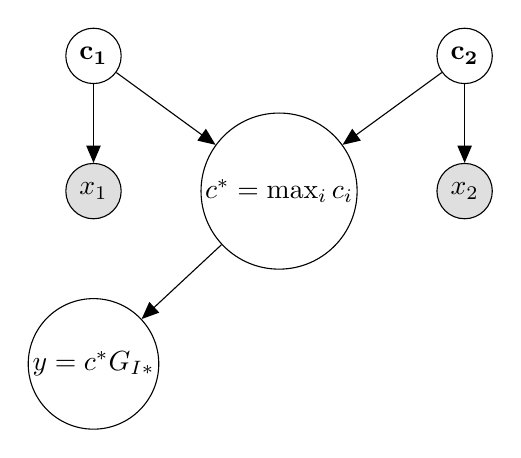
\begin{tikzpicture}

  % Define nodes
  \node[obs]                              (x_1) {$x_1$};
  \node[latent, right=of x_1]   (c_max) {$c^* = \max_i c_i$};
  \node[latent, below=of x_1]  (y) {$y = c^*G_{I*}$};
  \node[obs, right=of c_max]   (x_2) {$x_2$};
  \node[latent, above=of x_1] (c_1) {$\mathbf{c_1}$};
  \node[latent, above=of x_2]  (c_2) {$\mathbf{c_2}$};

  % Connect the nodes
  \edge {c_1} {x_1} ; 
  \edge {c_2} {x_2} ; 
  \edge {c_1} {c_max} ; 
  \edge {c_2} {c_max} ; 
  \edge {c_max} {y} ; 

\end{tikzpicture}
\\
\\
\begin{equation}
\begin{aligned}
p(y|x_1, x_2) & \propto p(x_1, x_2, c_1, c_2 | y)\\
& = \iint p(x_1|c_1) p(x_2|c_2) p(y | c_1, c_2) d c_1, d c_2 \\
& = \iint p(x_1|c_1) p(x_2|c_2) p(y | c_1, c_2) d c_1, d c_2 \\
& = \iint \mathcal{N}(x_1; c_1, \sigma^2) \mathcal{N}(x_2; c_2, \sigma^2) \delta(y - \max_i c_iG_i) dc_1 dc_2 \\
& = \iint_{c_1 \geq c_2} \mathcal{N}(x_1; c_1, \sigma^2) \mathcal{N}(x_2; c_2, \sigma^2) \delta(y - c_1G_1) dc_1 dc_2 \\
& \phantom{{}=1} + \iint_{c_1 < c_2} \mathcal{N}(x_1; c_1, \sigma^2) \mathcal{N}(x_2; c_2, \sigma^2) \delta(y - c_2G_2) dc_1 dc_2\\
\\
w_1 & = \int\limits_{-\infty}^{\infty}(\int\limits_{-\infty}^{c_1} \mathcal{N}(x_1; c_1, \sigma^2) \mathcal{N}(x_2; c_2, \sigma^2) dc_2) c_1 dc_1 ???\\
& = \frac{1}{2} + \frac{1}{2}\int c_1 \mathcal{N}(x_1; c_1, \sigma^2) \erf (\frac{c_1 - x_2}{\sigma \sqrt{2}} d c_1)
\end{aligned}
\end{equation}

\end{document}